\documentclass[1p]{elsarticle_modified}
%\bibliographystyle{elsarticle-num}

%\usepackage[colorlinks]{hyperref}
%\usepackage{abbrmath_seonhwa} %\Abb, \Ascr, \Acal ,\Abf, \Afrak
\usepackage{amsfonts}
\usepackage{amssymb}
\usepackage{amsmath}
\usepackage{amsthm}
\usepackage{scalefnt}
\usepackage{amsbsy}
\usepackage{kotex}
\usepackage{caption}
\usepackage{subfig}
\usepackage{color}
\usepackage{graphicx}
\usepackage{xcolor} %% white, black, red, green, blue, cyan, magenta, yellow
\usepackage{float}
\usepackage{setspace}
\usepackage{hyperref}

\usepackage{tikz}
\usetikzlibrary{arrows}

\usepackage{multirow}
\usepackage{array} % fixed length table
\usepackage{hhline}

%%%%%%%%%%%%%%%%%%%%%
\makeatletter
\renewcommand*\env@matrix[1][\arraystretch]{%
	\edef\arraystretch{#1}%
	\hskip -\arraycolsep
	\let\@ifnextchar\new@ifnextchar
	\array{*\c@MaxMatrixCols c}}
\makeatother %https://tex.stackexchange.com/questions/14071/how-can-i-increase-the-line-spacing-in-a-matrix
%%%%%%%%%%%%%%%

\usepackage[normalem]{ulem}

\newcommand{\msout}[1]{\ifmmode\text{\sout{\ensuremath{#1}}}\else\sout{#1}\fi}
%SOURCE: \msout is \stkout macro in https://tex.stackexchange.com/questions/20609/strikeout-in-math-mode

\newcommand{\cancel}[1]{
	\ifmmode
	{\color{red}\msout{#1}}
	\else
	{\color{red}\sout{#1}}
	\fi
}

\newcommand{\add}[1]{
	{\color{blue}\uwave{#1}}
}

\newcommand{\replace}[2]{
	\ifmmode
	{\color{red}\msout{#1}}{\color{blue}\uwave{#2}}
	\else
	{\color{red}\sout{#1}}{\color{blue}\uwave{#2}}
	\fi
}

\newcommand{\Sol}{\mathcal{S}} %segment
\newcommand{\D}{D} %diagram
\newcommand{\A}{\mathcal{A}} %arc


%%%%%%%%%%%%%%%%%%%%%%%%%%%%%5 test

\def\sl{\operatorname{\textup{SL}}(2,\Cbb)}
\def\psl{\operatorname{\textup{PSL}}(2,\Cbb)}
\def\quan{\mkern 1mu \triangleright \mkern 1mu}

\theoremstyle{definition}
\newtheorem{thm}{Theorem}[section]
\newtheorem{prop}[thm]{Proposition}
\newtheorem{lem}[thm]{Lemma}
\newtheorem{ques}[thm]{Question}
\newtheorem{cor}[thm]{Corollary}
\newtheorem{defn}[thm]{Definition}
\newtheorem{exam}[thm]{Example}
\newtheorem{rmk}[thm]{Remark}
\newtheorem{alg}[thm]{Algorithm}

\newcommand{\I}{\sqrt{-1}}
\begin{document}

%\begin{frontmatter}
%
%\title{Boundary parabolic representations of knots up to 8 crossings}
%
%%% Group authors per affiliation:
%\author{Yunhi Cho} 
%\address{Department of Mathematics, University of Seoul, Seoul, Korea}
%\ead{yhcho@uos.ac.kr}
%
%
%\author{Seonhwa Kim} %\fnref{s_kim}}
%\address{Center for Geometry and Physics, Institute for Basic Science, Pohang, 37673, Korea}
%\ead{ryeona17@ibs.re.kr}
%
%\author{Hyuk Kim}
%\address{Department of Mathematical Sciences, Seoul National University, Seoul 08826, Korea}
%\ead{hyukkim@snu.ac.kr}
%
%\author{Seokbeom Yoon}
%\address{Department of Mathematical Sciences, Seoul National University, Seoul, 08826,  Korea}
%\ead{sbyoon15@snu.ac.kr}
%
%\begin{abstract}
%We find all boundary parabolic representation of knots up to 8 crossings.
%
%\end{abstract}
%\begin{keyword}
%    \MSC[2010] 57M25 
%\end{keyword}
%
%\end{frontmatter}

%\linenumbers
%\tableofcontents
%
\newcommand\colored[1]{\textcolor{white}{\rule[-0.35ex]{0.8em}{1.4ex}}\kern-0.8em\color{red} #1}%
%\newcommand\colored[1]{\textcolor{white}{ #1}\kern-2.17ex	\textcolor{white}{ #1}\kern-1.81ex	\textcolor{white}{ #1}\kern-2.15ex\color{red}#1	}

{\Large $\underline{11a_{219}~(K11a_{219})}$}

\setlength{\tabcolsep}{10pt}
\renewcommand{\arraystretch}{1.6}
\vspace{1cm}\begin{tabular}{m{100pt}>{\centering\arraybackslash}m{274pt}}
\multirow{5}{120pt}{
	\centering
	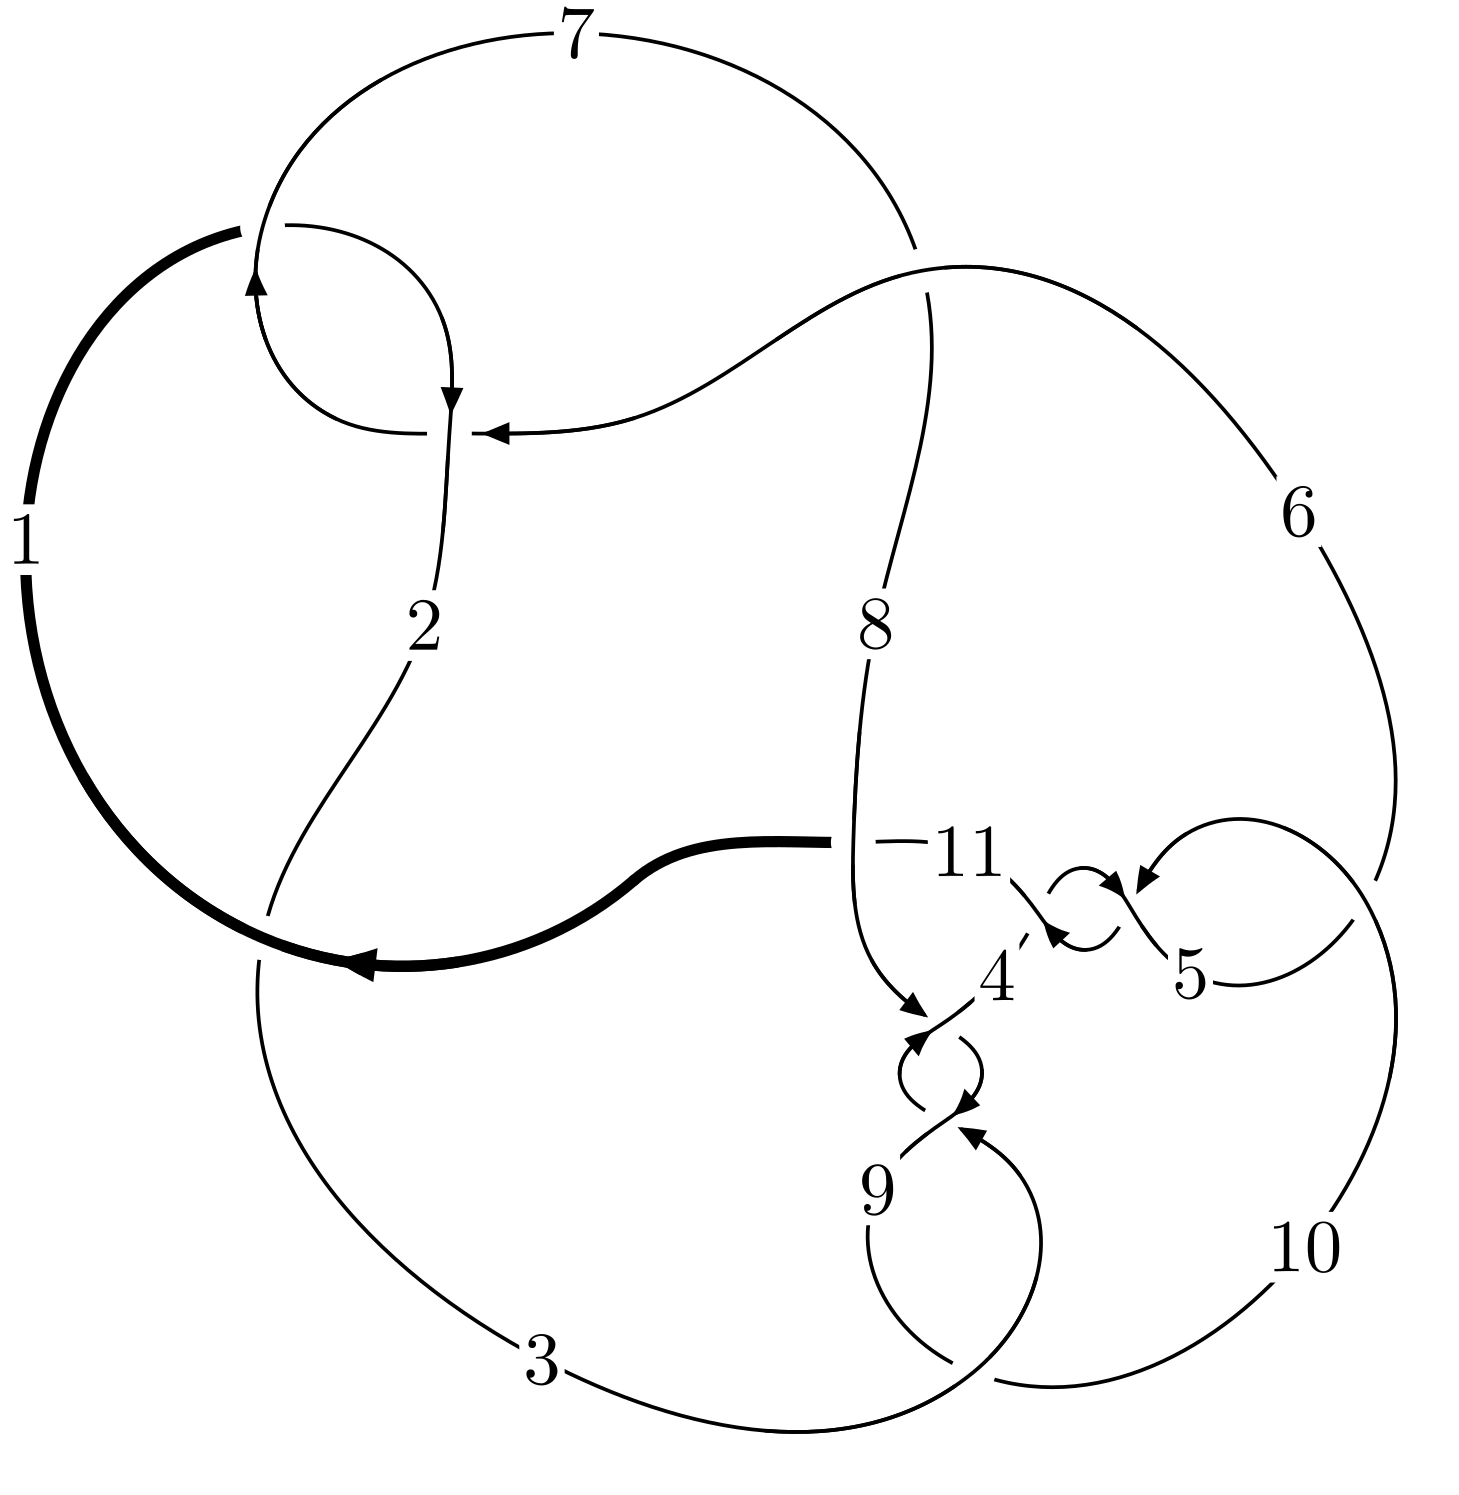
\includegraphics[width=112pt]{../../../GIT/diagram.site/Diagrams/png/468_11a_219.png}\\
\ \ \ A knot diagram\footnotemark}&
\allowdisplaybreaks
\textbf{Linearized knot diagam} \\
\cline{2-2}
 &
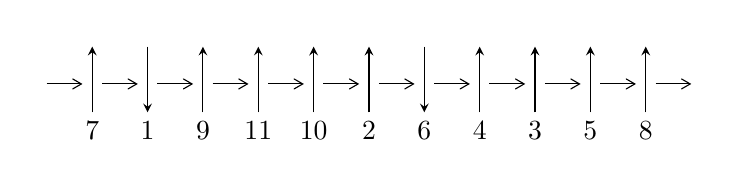
\begin{tikzpicture}[x=20pt, y=17pt]
	% nodes
	\node (C0) at (0, 0) {};
	\node (C1) at (1, 0) {};
	\node (C1U) at (1, +1) {};
	\node (C1D) at (1, -1) {7};

	\node (C2) at (2, 0) {};
	\node (C2U) at (2, +1) {};
	\node (C2D) at (2, -1) {1};

	\node (C3) at (3, 0) {};
	\node (C3U) at (3, +1) {};
	\node (C3D) at (3, -1) {9};

	\node (C4) at (4, 0) {};
	\node (C4U) at (4, +1) {};
	\node (C4D) at (4, -1) {11};

	\node (C5) at (5, 0) {};
	\node (C5U) at (5, +1) {};
	\node (C5D) at (5, -1) {10};

	\node (C6) at (6, 0) {};
	\node (C6U) at (6, +1) {};
	\node (C6D) at (6, -1) {2};

	\node (C7) at (7, 0) {};
	\node (C7U) at (7, +1) {};
	\node (C7D) at (7, -1) {6};

	\node (C8) at (8, 0) {};
	\node (C8U) at (8, +1) {};
	\node (C8D) at (8, -1) {4};

	\node (C9) at (9, 0) {};
	\node (C9U) at (9, +1) {};
	\node (C9D) at (9, -1) {3};

	\node (C10) at (10, 0) {};
	\node (C10U) at (10, +1) {};
	\node (C10D) at (10, -1) {5};

	\node (C11) at (11, 0) {};
	\node (C11U) at (11, +1) {};
	\node (C11D) at (11, -1) {8};
	\node (C12) at (12, 0) {};

	% arrows
	\draw[->,>={angle 60}]
	(C0) edge (C1) (C1) edge (C2) (C2) edge (C3) (C3) edge (C4) (C4) edge (C5) (C5) edge (C6) (C6) edge (C7) (C7) edge (C8) (C8) edge (C9) (C9) edge (C10) (C10) edge (C11) (C11) edge (C12) ;	\draw[->,>=stealth]
	(C1D) edge (C1U) (C2U) edge (C2D) (C3D) edge (C3U) (C4D) edge (C4U) (C5D) edge (C5U) (C6D) edge (C6U) (C7U) edge (C7D) (C8D) edge (C8U) (C9D) edge (C9U) (C10D) edge (C10U) (C11D) edge (C11U) ;
	\end{tikzpicture} \\
\hhline{~~} \\& 
\textbf{Solving Sequence} \\ \cline{2-2} 
 &
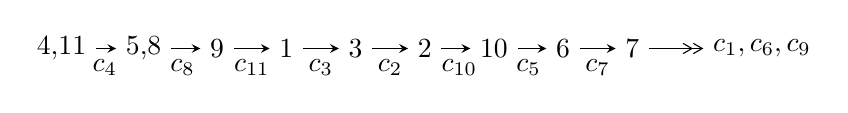
\begin{tikzpicture}[x=25pt, y=7pt]
	% node
	\node (A0) at (-1/8, 0) {4,11};
	\node (A1) at (17/16, 0) {5,8};
	\node (A2) at (17/8, 0) {9};
	\node (A3) at (25/8, 0) {1};
	\node (A4) at (33/8, 0) {3};
	\node (A5) at (41/8, 0) {2};
	\node (A6) at (49/8, 0) {10};
	\node (A7) at (57/8, 0) {6};
	\node (A8) at (65/8, 0) {7};
	\node (C1) at (1/2, -1) {$c_{4}$};
	\node (C2) at (13/8, -1) {$c_{8}$};
	\node (C3) at (21/8, -1) {$c_{11}$};
	\node (C4) at (29/8, -1) {$c_{3}$};
	\node (C5) at (37/8, -1) {$c_{2}$};
	\node (C6) at (45/8, -1) {$c_{10}$};
	\node (C7) at (53/8, -1) {$c_{5}$};
	\node (C8) at (61/8, -1) {$c_{7}$};
	\node (A9) at (10, 0) {$c_{1},c_{6},c_{9}$};

	% edge
	\draw[->,>=stealth]	
	(A0) edge (A1) (A1) edge (A2) (A2) edge (A3) (A3) edge (A4) (A4) edge (A5) (A5) edge (A6) (A6) edge (A7) (A7) edge (A8) ;
	\draw[->>,>={angle 60}]	
	(A8) edge (A9);
\end{tikzpicture} \\ 

\end{tabular} \\

\footnotetext{
The image of knot diagram is generated by the software ``\textbf{Draw programme}" developed by Andrew Bartholomew(\url{http://www.layer8.co.uk/maths/draw/index.htm\#Running-draw}), where we modified some parts for our purpose(\url{https://github.com/CATsTAILs/LinksPainter}).
}\phantom \\ \newline 
\centering \textbf{Ideals for irreducible components\footnotemark of $X_{\text{par}}$} 
 
\begin{align*}
I^u_{1}&=\langle 
b- u,\;- u^{20}- u^{19}+\cdots+8 a+1,\;u^{21}+13 u^{19}+\cdots+12 u^3-1\rangle \\
I^u_{2}&=\langle 
-2624442537 u^{27}+1988686630 u^{26}+\cdots+16455396275 b-10223804083,\\
\phantom{I^u_{2}}&\phantom{= \langle  }19079838812 u^{27}-18444082905 u^{26}+\cdots+16455396275 a+108956181733,\\
\phantom{I^u_{2}}&\phantom{= \langle  }u^{28}- u^{27}+\cdots+6 u+1\rangle \\
I^u_{3}&=\langle 
b+u,\;a^3+a^2+2 a+1,\;u^2+1\rangle \\
\\
\end{align*}
\raggedright * 3 irreducible components of $\dim_{\mathbb{C}}=0$, with total 55 representations.\\
\footnotetext{All coefficients of polynomials are rational numbers. But the coefficients are sometimes approximated in decimal forms when there is not enough margin.}
\newpage
\renewcommand{\arraystretch}{1}
\centering \section*{I. $I^u_{1}= \langle b- u,\;- u^{20}- u^{19}+\cdots+8 a+1,\;u^{21}+13 u^{19}+\cdots+12 u^3-1 \rangle$}
\flushleft \textbf{(i) Arc colorings}\\
\begin{tabular}{m{7pt} m{180pt} m{7pt} m{180pt} }
\flushright $a_{4}=$&$\begin{pmatrix}1\\0\end{pmatrix}$ \\
\flushright $a_{11}=$&$\begin{pmatrix}0\\u\end{pmatrix}$ \\
\flushright $a_{5}=$&$\begin{pmatrix}1\\- u^2\end{pmatrix}$ \\
\flushright $a_{8}=$&$\begin{pmatrix}\frac{1}{8} u^{20}+\frac{1}{8} u^{19}+\cdots-\frac{25}{8} u-\frac{1}{8}\\u\end{pmatrix}$ \\
\flushright $a_{9}=$&$\begin{pmatrix}\frac{1}{8} u^{20}+\frac{1}{8} u^{19}+\cdots-\frac{17}{8} u-\frac{1}{8}\\u\end{pmatrix}$ \\
\flushright $a_{1}=$&$\begin{pmatrix}\frac{1}{8} u^{20}-\frac{1}{8} u^{19}+\cdots-\frac{3}{8} u-\frac{1}{8}\\-\frac{1}{8} u^{20}-\frac{1}{8} u^{19}+\cdots+\frac{9}{8} u+\frac{1}{8}\end{pmatrix}$ \\
\flushright $a_{3}=$&$\begin{pmatrix}\frac{1}{8} u^{20}-\frac{1}{8} u^{19}+\cdots-\frac{1}{8} u+\frac{9}{8}\\u^2\end{pmatrix}$ \\
\flushright $a_{2}=$&$\begin{pmatrix}-\frac{3}{8} u^{20}+\frac{5}{8} u^{19}+\cdots+\frac{7}{8} u-\frac{1}{8}\\\frac{1}{4} u^{18}-\frac{1}{4} u^{17}+\cdots-\frac{1}{4} u+\frac{1}{4}\end{pmatrix}$ \\
\flushright $a_{10}=$&$\begin{pmatrix}- u\\u^3+u\end{pmatrix}$ \\
\flushright $a_{6}=$&$\begin{pmatrix}u^2+1\\- u^4-2 u^2\end{pmatrix}$ \\
\flushright $a_{7}=$&$\begin{pmatrix}\frac{1}{8} u^{20}+\frac{1}{8} u^{19}+\cdots-\frac{17}{8} u-\frac{1}{8}\\-\frac{1}{8} u^{20}-\frac{1}{8} u^{19}+\cdots+\frac{9}{8} u+\frac{1}{8}\end{pmatrix}$\\ \flushright $a_{7}=$&$\begin{pmatrix}\frac{1}{8} u^{20}+\frac{1}{8} u^{19}+\cdots-\frac{17}{8} u-\frac{1}{8}\\-\frac{1}{8} u^{20}-\frac{1}{8} u^{19}+\cdots+\frac{9}{8} u+\frac{1}{8}\end{pmatrix}$\\&\end{tabular}
\flushleft \textbf{(ii) Obstruction class $= -1$}\\~\\
\flushleft \textbf{(iii) Cusp Shapes $= \frac{5}{2} u^{20}+u^{19}+\frac{65}{2} u^{18}+15 u^{17}+177 u^{16}+\frac{181}{2} u^{15}+\frac{1023}{2} u^{14}+280 u^{13}+806 u^{12}+\frac{907}{2} u^{11}+599 u^{10}+316 u^9+\frac{119}{2} u^8-\frac{27}{2} u^7-88 u^6-49 u^5+\frac{99}{2} u^4+\frac{129}{2} u^3+17 u^2+12 u+\frac{11}{2}$}\\~\\
\newpage\renewcommand{\arraystretch}{1}
\flushleft \textbf{(iv) u-Polynomials at the component}\newline \\
\begin{tabular}{m{50pt}|m{274pt}}
Crossings & \hspace{64pt}u-Polynomials at each crossing \\
\hline $$\begin{aligned}c_{1},c_{6}\end{aligned}$$&$\begin{aligned}
&u^{21}+3 u^{20}+\cdots+3 u-2
\end{aligned}$\\
\hline $$\begin{aligned}c_{2},c_{7}\end{aligned}$$&$\begin{aligned}
&u^{21}+7 u^{20}+\cdots+21 u-4
\end{aligned}$\\
\hline $$\begin{aligned}c_{3},c_{4},c_{5}\\c_{8},c_{9},c_{10}\end{aligned}$$&$\begin{aligned}
&u^{21}+13 u^{19}+\cdots+12 u^3-1
\end{aligned}$\\
\hline $$\begin{aligned}c_{11}\end{aligned}$$&$\begin{aligned}
&u^{21}-15 u^{20}+\cdots+2103 u-266
\end{aligned}$\\
\hline
\end{tabular}\\~\\
\newpage\renewcommand{\arraystretch}{1}
\flushleft \textbf{(v) Riley Polynomials at the component}\newline \\
\begin{tabular}{m{50pt}|m{274pt}}
Crossings & \hspace{64pt}Riley Polynomials at each crossing \\
\hline $$\begin{aligned}c_{1},c_{6}\end{aligned}$$&$\begin{aligned}
&y^{21}+7 y^{20}+\cdots+21 y-4
\end{aligned}$\\
\hline $$\begin{aligned}c_{2},c_{7}\end{aligned}$$&$\begin{aligned}
&y^{21}+15 y^{20}+\cdots+1137 y-16
\end{aligned}$\\
\hline $$\begin{aligned}c_{3},c_{4},c_{5}\\c_{8},c_{9},c_{10}\end{aligned}$$&$\begin{aligned}
&y^{21}+26 y^{20}+\cdots+24 y^2-1
\end{aligned}$\\
\hline $$\begin{aligned}c_{11}\end{aligned}$$&$\begin{aligned}
&y^{21}+3 y^{20}+\cdots+343765 y-70756
\end{aligned}$\\
\hline
\end{tabular}\\~\\
\newpage\flushleft \textbf{(vi) Complex Volumes and Cusp Shapes}
$$\begin{array}{c|c|c}  
\text{Solutions to }I^u_{1}& \I (\text{vol} + \sqrt{-1}CS) & \text{Cusp shape}\\
 \hline 
\begin{aligned}
u &= -0.626749 + 0.333863 I \\
a &= \phantom{-}1.66451 - 0.51604 I \\
b &= -0.626749 + 0.333863 I\end{aligned}
 & \phantom{-}2.49171 - 5.86529 I & \phantom{-}9.54952 + 8.01834 I \\ \hline\begin{aligned}
u &= -0.626749 - 0.333863 I \\
a &= \phantom{-}1.66451 + 0.51604 I \\
b &= -0.626749 - 0.333863 I\end{aligned}
 & \phantom{-}2.49171 + 5.86529 I & \phantom{-}9.54952 - 8.01834 I \\ \hline\begin{aligned}
u &= \phantom{-}0.629746 + 0.248411 I \\
a &= -1.60683 - 0.39158 I \\
b &= \phantom{-}0.629746 + 0.248411 I\end{aligned}
 & \phantom{-}3.16640 + 0.40908 I & \phantom{-}11.72672 - 2.09398 I \\ \hline\begin{aligned}
u &= \phantom{-}0.629746 - 0.248411 I \\
a &= -1.60683 + 0.39158 I \\
b &= \phantom{-}0.629746 - 0.248411 I\end{aligned}
 & \phantom{-}3.16640 - 0.40908 I & \phantom{-}11.72672 + 2.09398 I \\ \hline\begin{aligned}
u &= -0.020126 + 1.386560 I \\
a &= \phantom{-}0.15798 + 1.61235 I \\
b &= -0.020126 + 1.386560 I\end{aligned}
 & -3.09312 - 3.11987 I & \phantom{-}1.81385 + 2.72222 I \\ \hline\begin{aligned}
u &= -0.020126 - 1.386560 I \\
a &= \phantom{-}0.15798 - 1.61235 I \\
b &= -0.020126 - 1.386560 I\end{aligned}
 & -3.09312 + 3.11987 I & \phantom{-}1.81385 - 2.72222 I \\ \hline\begin{aligned}
u &= -0.049869 + 0.513457 I \\
a &= \phantom{-}0.28009 - 1.88738 I \\
b &= -0.049869 + 0.513457 I\end{aligned}
 & \phantom{-}1.38918 + 2.68088 I & \phantom{-}7.84813 - 2.28119 I \\ \hline\begin{aligned}
u &= -0.049869 - 0.513457 I \\
a &= \phantom{-}0.28009 + 1.88738 I \\
b &= -0.049869 - 0.513457 I\end{aligned}
 & \phantom{-}1.38918 - 2.68088 I & \phantom{-}7.84813 + 2.28119 I \\ \hline\begin{aligned}
u &= -0.358971 + 0.369522 I \\
a &= \phantom{-}1.22004 - 0.88408 I \\
b &= -0.358971 + 0.369522 I\end{aligned}
 & -1.99273 - 1.21629 I & \phantom{-}2.57418 + 5.92996 I \\ \hline\begin{aligned}
u &= -0.358971 - 0.369522 I \\
a &= \phantom{-}1.22004 + 0.88408 I \\
b &= -0.358971 - 0.369522 I\end{aligned}
 & -1.99273 + 1.21629 I & \phantom{-}2.57418 - 5.92996 I\\
 \hline 
 \end{array}$$\newpage$$\begin{array}{c|c|c}  
\text{Solutions to }I^u_{1}& \I (\text{vol} + \sqrt{-1}CS) & \text{Cusp shape}\\
 \hline 
\begin{aligned}
u &= -0.31097 + 1.49970 I \\
a &= \phantom{-}1.257710 + 0.336801 I \\
b &= -0.31097 + 1.49970 I\end{aligned}
 & -8.25449 - 7.57688 I & \phantom{-}3.21336 + 3.12167 I \\ \hline\begin{aligned}
u &= -0.31097 - 1.49970 I \\
a &= \phantom{-}1.257710 - 0.336801 I \\
b &= -0.31097 - 1.49970 I\end{aligned}
 & -8.25449 + 7.57688 I & \phantom{-}3.21336 - 3.12167 I \\ \hline\begin{aligned}
u &= -0.18915 + 1.52129 I \\
a &= \phantom{-}0.833836 + 0.568249 I \\
b &= -0.18915 + 1.52129 I\end{aligned}
 & -10.20410 - 4.07649 I & \phantom{-}2.56533 + 2.84794 I \\ \hline\begin{aligned}
u &= -0.18915 - 1.52129 I \\
a &= \phantom{-}0.833836 - 0.568249 I \\
b &= -0.18915 - 1.52129 I\end{aligned}
 & -10.20410 + 4.07649 I & \phantom{-}2.56533 - 2.84794 I \\ \hline\begin{aligned}
u &= \phantom{-}0.33859 + 1.51855 I \\
a &= -1.273830 + 0.223483 I \\
b &= \phantom{-}0.33859 + 1.51855 I\end{aligned}
 & -9.5708 + 13.4578 I & \phantom{-}1.56507 - 7.58317 I \\ \hline\begin{aligned}
u &= \phantom{-}0.33859 - 1.51855 I \\
a &= -1.273830 - 0.223483 I \\
b &= \phantom{-}0.33859 - 1.51855 I\end{aligned}
 & -9.5708 - 13.4578 I & \phantom{-}1.56507 + 7.58317 I \\ \hline\begin{aligned}
u &= \phantom{-}0.14072 + 1.58052 I \\
a &= -0.556156 + 0.432838 I \\
b &= \phantom{-}0.14072 + 1.58052 I\end{aligned}
 & -12.61950 - 0.61749 I & -1.09619 + 1.91653 I \\ \hline\begin{aligned}
u &= \phantom{-}0.14072 - 1.58052 I \\
a &= -0.556156 - 0.432838 I \\
b &= \phantom{-}0.14072 - 1.58052 I\end{aligned}
 & -12.61950 + 0.61749 I & -1.09619 - 1.91653 I \\ \hline\begin{aligned}
u &= \phantom{-}0.25937 + 1.56915 I \\
a &= -0.961257 + 0.271014 I \\
b &= \phantom{-}0.25937 + 1.56915 I\end{aligned}
 & -15.0783 + 6.7163 I & -2.88981 - 3.97813 I \\ \hline\begin{aligned}
u &= \phantom{-}0.25937 - 1.56915 I \\
a &= -0.961257 - 0.271014 I \\
b &= \phantom{-}0.25937 - 1.56915 I\end{aligned}
 & -15.0783 - 6.7163 I & -2.88981 + 3.97813 I\\
 \hline 
 \end{array}$$\newpage$$\begin{array}{c|c|c}  
\text{Solutions to }I^u_{1}& \I (\text{vol} + \sqrt{-1}CS) & \text{Cusp shape}\\
 \hline 
\begin{aligned}
u &= \phantom{-}0.374847\phantom{ +0.000000I} \\
a &= -1.03218\phantom{ +0.000000I} \\
b &= \phantom{-}0.374847\phantom{ +0.000000I}\end{aligned}
 & \phantom{-}0.610872\phantom{ +0.000000I} & \phantom{-}16.2600\phantom{ +0.000000I}\\
 \hline 
 \end{array}$$\newpage\newpage\renewcommand{\arraystretch}{1}
\centering \section*{II. $I^u_{2}= \langle -2.62\times10^{9} u^{27}+1.99\times10^{9} u^{26}+\cdots+1.65\times10^{10} b-1.02\times10^{10},\;1.91\times10^{10} u^{27}-1.84\times10^{10} u^{26}+\cdots+1.65\times10^{10} a+1.09\times10^{11},\;u^{28}- u^{27}+\cdots+6 u+1 \rangle$}
\flushleft \textbf{(i) Arc colorings}\\
\begin{tabular}{m{7pt} m{180pt} m{7pt} m{180pt} }
\flushright $a_{4}=$&$\begin{pmatrix}1\\0\end{pmatrix}$ \\
\flushright $a_{11}=$&$\begin{pmatrix}0\\u\end{pmatrix}$ \\
\flushright $a_{5}=$&$\begin{pmatrix}1\\- u^2\end{pmatrix}$ \\
\flushright $a_{8}=$&$\begin{pmatrix}-1.15949 u^{27}+1.12085 u^{26}+\cdots-31.4295 u-6.62130\\0.159488 u^{27}-0.120853 u^{26}+\cdots+5.42946 u+0.621304\end{pmatrix}$ \\
\flushright $a_{9}=$&$\begin{pmatrix}- u^{27}+u^{26}+\cdots-26 u-6\\0.159488 u^{27}-0.120853 u^{26}+\cdots+5.42946 u+0.621304\end{pmatrix}$ \\
\flushright $a_{1}=$&$\begin{pmatrix}-1.49816 u^{27}+1.73027 u^{26}+\cdots-37.4676 u-7.20397\\0.338676 u^{27}-0.609413 u^{26}+\cdots+7.03817 u+0.582669\end{pmatrix}$ \\
\flushright $a_{3}=$&$\begin{pmatrix}-0.621304 u^{27}+0.780792 u^{26}+\cdots-15.8797 u+2.70164\\-0.0386351 u^{27}-0.140553 u^{26}+\cdots+0.335626 u-0.840512\end{pmatrix}$ \\
\flushright $a_{2}=$&$\begin{pmatrix}-0.251205 u^{27}+0.244139 u^{26}+\cdots-4.73991 u-4.26868\\0.464204 u^{27}-0.736552 u^{26}+\cdots+3.57003 u+0.996329\end{pmatrix}$ \\
\flushright $a_{10}=$&$\begin{pmatrix}- u\\u^3+u\end{pmatrix}$ \\
\flushright $a_{6}=$&$\begin{pmatrix}u^2+1\\- u^4-2 u^2\end{pmatrix}$ \\
\flushright $a_{7}=$&$\begin{pmatrix}-0.860293 u^{27}+0.936481 u^{26}+\cdots-23.2248 u-5.89350\\0.0244857 u^{27}-0.155424 u^{26}+\cdots+4.35668 u+0.358891\end{pmatrix}$\\ \flushright $a_{7}=$&$\begin{pmatrix}-0.860293 u^{27}+0.936481 u^{26}+\cdots-23.2248 u-5.89350\\0.0244857 u^{27}-0.155424 u^{26}+\cdots+4.35668 u+0.358891\end{pmatrix}$\\&\end{tabular}
\flushleft \textbf{(ii) Obstruction class $= -1$}\\~\\
\flushleft \textbf{(iii) Cusp Shapes $= \frac{7485203784}{16455396275} u^{27}-\frac{4244606112}{3291079255} u^{26}+\cdots-\frac{308226995468}{16455396275} u+\frac{121631108806}{16455396275}$}\\~\\
\newpage\renewcommand{\arraystretch}{1}
\flushleft \textbf{(iv) u-Polynomials at the component}\newline \\
\begin{tabular}{m{50pt}|m{274pt}}
Crossings & \hspace{64pt}u-Polynomials at each crossing \\
\hline $$\begin{aligned}c_{1},c_{6}\end{aligned}$$&$\begin{aligned}
&(u^{14}- u^{13}+\cdots+u+1)^{2}
\end{aligned}$\\
\hline $$\begin{aligned}c_{2},c_{7},c_{11}\end{aligned}$$&$\begin{aligned}
&(u^{14}+5 u^{13}+\cdots+3 u+1)^{2}
\end{aligned}$\\
\hline $$\begin{aligned}c_{3},c_{4},c_{5}\\c_{8},c_{9},c_{10}\end{aligned}$$&$\begin{aligned}
&u^{28}- u^{27}+\cdots+6 u+1
\end{aligned}$\\
\hline
\end{tabular}\\~\\
\newpage\renewcommand{\arraystretch}{1}
\flushleft \textbf{(v) Riley Polynomials at the component}\newline \\
\begin{tabular}{m{50pt}|m{274pt}}
Crossings & \hspace{64pt}Riley Polynomials at each crossing \\
\hline $$\begin{aligned}c_{1},c_{6}\end{aligned}$$&$\begin{aligned}
&(y^{14}+5 y^{13}+\cdots+3 y+1)^{2}
\end{aligned}$\\
\hline $$\begin{aligned}c_{2},c_{7},c_{11}\end{aligned}$$&$\begin{aligned}
&(y^{14}+9 y^{13}+\cdots+15 y+1)^{2}
\end{aligned}$\\
\hline $$\begin{aligned}c_{3},c_{4},c_{5}\\c_{8},c_{9},c_{10}\end{aligned}$$&$\begin{aligned}
&y^{28}+23 y^{27}+\cdots+16 y+1
\end{aligned}$\\
\hline
\end{tabular}\\~\\
\newpage\flushleft \textbf{(vi) Complex Volumes and Cusp Shapes}
$$\begin{array}{c|c|c}  
\text{Solutions to }I^u_{2}& \I (\text{vol} + \sqrt{-1}CS) & \text{Cusp shape}\\
 \hline 
\begin{aligned}
u &= \phantom{-}0.903414 + 0.423724 I \\
a &= \phantom{-}1.12702 + 1.02376 I \\
b &= -0.21970 - 1.44931 I\end{aligned}
 & -3.28987 + 8.93586 I & \phantom{-}4.00000 - 7.26077 I \\ \hline\begin{aligned}
u &= \phantom{-}0.903414 - 0.423724 I \\
a &= \phantom{-}1.12702 - 1.02376 I \\
b &= -0.21970 + 1.44931 I\end{aligned}
 & -3.28987 - 8.93586 I & \phantom{-}4.00000 + 7.26077 I \\ \hline\begin{aligned}
u &= \phantom{-}0.821921 + 0.594799 I \\
a &= \phantom{-}0.892891 + 0.877803 I \\
b &= -0.09440 - 1.45565 I\end{aligned}
 & -7.93259 + 2.76747 I & -1.41762 - 3.21377 I \\ \hline\begin{aligned}
u &= \phantom{-}0.821921 - 0.594799 I \\
a &= \phantom{-}0.892891 - 0.877803 I \\
b &= -0.09440 + 1.45565 I\end{aligned}
 & -7.93259 - 2.76747 I & -1.41762 + 3.21377 I \\ \hline\begin{aligned}
u &= \phantom{-}0.709754 + 0.808180 I \\
a &= \phantom{-}0.550947 + 0.736144 I \\
b &= \phantom{-}0.06255 - 1.43472 I\end{aligned}
 & -4.48016 - 3.41271 I & \phantom{-}1.89400 + 2.62516 I \\ \hline\begin{aligned}
u &= \phantom{-}0.709754 - 0.808180 I \\
a &= \phantom{-}0.550947 - 0.736144 I \\
b &= \phantom{-}0.06255 + 1.43472 I\end{aligned}
 & -4.48016 + 3.41271 I & \phantom{-}1.89400 - 2.62516 I \\ \hline\begin{aligned}
u &= -0.830600 + 0.398708 I \\
a &= -1.18688 + 0.93008 I \\
b &= \phantom{-}0.20839 - 1.39977 I\end{aligned}
 & -2.09958 - 3.41271 I & \phantom{-}6.10600 + 2.62516 I \\ \hline\begin{aligned}
u &= -0.830600 - 0.398708 I \\
a &= -1.18688 - 0.93008 I \\
b &= \phantom{-}0.20839 + 1.39977 I\end{aligned}
 & -2.09958 + 3.41271 I & \phantom{-}6.10600 - 2.62516 I \\ \hline\begin{aligned}
u &= \phantom{-}0.081869 + 0.917517 I \\
a &= \phantom{-}0.228572 - 1.240560 I \\
b &= -0.132090 + 0.159270 I\end{aligned}
 & \phantom{-}1.35286 + 2.76747 I & \phantom{-}9.41762 - 3.21377 I \\ \hline\begin{aligned}
u &= \phantom{-}0.081869 - 0.917517 I \\
a &= \phantom{-}0.228572 + 1.240560 I \\
b &= -0.132090 - 0.159270 I\end{aligned}
 & \phantom{-}1.35286 - 2.76747 I & \phantom{-}9.41762 + 3.21377 I\\
 \hline 
 \end{array}$$\newpage$$\begin{array}{c|c|c}  
\text{Solutions to }I^u_{2}& \I (\text{vol} + \sqrt{-1}CS) & \text{Cusp shape}\\
 \hline 
\begin{aligned}
u &= -0.428554 + 0.809341 I \\
a &= -0.422476 + 0.298820 I \\
b &= -0.088503 - 1.263820 I\end{aligned}
 & -3.31269 - 1.37770 I & \phantom{-}3.11410 + 4.12207 I \\ \hline\begin{aligned}
u &= -0.428554 - 0.809341 I \\
a &= -0.422476 - 0.298820 I \\
b &= -0.088503 + 1.263820 I\end{aligned}
 & -3.31269 + 1.37770 I & \phantom{-}3.11410 - 4.12207 I \\ \hline\begin{aligned}
u &= -0.503703 + 0.626414 I \\
a &= -0.789243 + 0.320757 I \\
b &= \phantom{-}0.009651 - 1.290270 I\end{aligned}
 & -3.26705 - 1.37770 I & \phantom{-}4.88590 + 4.12207 I \\ \hline\begin{aligned}
u &= -0.503703 - 0.626414 I \\
a &= -0.789243 - 0.320757 I \\
b &= \phantom{-}0.009651 + 1.290270 I\end{aligned}
 & -3.26705 + 1.37770 I & \phantom{-}4.88590 - 4.12207 I \\ \hline\begin{aligned}
u &= -0.088503 + 1.263820 I \\
a &= \phantom{-}0.373414 + 0.021953 I \\
b &= -0.428554 - 0.809341 I\end{aligned}
 & -3.31269 + 1.37770 I & \phantom{-}3.11410 - 4.12207 I \\ \hline\begin{aligned}
u &= -0.088503 - 1.263820 I \\
a &= \phantom{-}0.373414 - 0.021953 I \\
b &= -0.428554 + 0.809341 I\end{aligned}
 & -3.31269 - 1.37770 I & \phantom{-}3.11410 + 4.12207 I \\ \hline\begin{aligned}
u &= \phantom{-}0.009651 + 1.290270 I \\
a &= \phantom{-}0.509500 - 0.148574 I \\
b &= -0.503703 - 0.626414 I\end{aligned}
 & -3.26705 + 1.37770 I & \phantom{-}4.88590 - 4.12207 I \\ \hline\begin{aligned}
u &= \phantom{-}0.009651 - 1.290270 I \\
a &= \phantom{-}0.509500 + 0.148574 I \\
b &= -0.503703 + 0.626414 I\end{aligned}
 & -3.26705 - 1.37770 I & \phantom{-}4.88590 + 4.12207 I \\ \hline\begin{aligned}
u &= \phantom{-}0.20839 + 1.39977 I \\
a &= \phantom{-}0.934651 - 0.300202 I \\
b &= -0.830600 - 0.398708 I\end{aligned}
 & -2.09958 + 3.41271 I & \phantom{-}6.10600 - 2.62516 I \\ \hline\begin{aligned}
u &= \phantom{-}0.20839 - 1.39977 I \\
a &= \phantom{-}0.934651 + 0.300202 I \\
b &= -0.830600 + 0.398708 I\end{aligned}
 & -2.09958 - 3.41271 I & \phantom{-}6.10600 + 2.62516 I\\
 \hline 
 \end{array}$$\newpage$$\begin{array}{c|c|c}  
\text{Solutions to }I^u_{2}& \I (\text{vol} + \sqrt{-1}CS) & \text{Cusp shape}\\
 \hline 
\begin{aligned}
u &= \phantom{-}0.06255 + 1.43472 I \\
a &= -0.679426 + 0.112500 I \\
b &= \phantom{-}0.709754 - 0.808180 I\end{aligned}
 & -4.48016 + 3.41271 I & \phantom{-}1.89400 - 2.62516 I \\ \hline\begin{aligned}
u &= \phantom{-}0.06255 - 1.43472 I \\
a &= -0.679426 - 0.112500 I \\
b &= \phantom{-}0.709754 + 0.808180 I\end{aligned}
 & -4.48016 - 3.41271 I & \phantom{-}1.89400 + 2.62516 I \\ \hline\begin{aligned}
u &= -0.09440 + 1.45565 I \\
a &= -0.866285 - 0.089303 I \\
b &= \phantom{-}0.821921 - 0.594799 I\end{aligned}
 & -7.93259 - 2.76747 I & -1.41762 + 3.21377 I \\ \hline\begin{aligned}
u &= -0.09440 - 1.45565 I \\
a &= -0.866285 + 0.089303 I \\
b &= \phantom{-}0.821921 + 0.594799 I\end{aligned}
 & -7.93259 + 2.76747 I & -1.41762 - 3.21377 I \\ \hline\begin{aligned}
u &= -0.21970 + 1.44931 I \\
a &= -1.005660 - 0.250758 I \\
b &= \phantom{-}0.903414 - 0.423724 I\end{aligned}
 & -3.28987 - 8.93586 I & \phantom{-}4.00000 + 7.26077 I \\ \hline\begin{aligned}
u &= -0.21970 - 1.44931 I \\
a &= -1.005660 + 0.250758 I \\
b &= \phantom{-}0.903414 + 0.423724 I\end{aligned}
 & -3.28987 + 8.93586 I & \phantom{-}4.00000 - 7.26077 I \\ \hline\begin{aligned}
u &= -0.132090 + 0.159270 I \\
a &= -3.16703 - 4.63750 I \\
b &= \phantom{-}0.081869 + 0.917517 I\end{aligned}
 & \phantom{-}1.35286 + 2.76747 I & \phantom{-}9.41762 - 3.21377 I \\ \hline\begin{aligned}
u &= -0.132090 - 0.159270 I \\
a &= -3.16703 + 4.63750 I \\
b &= \phantom{-}0.081869 - 0.917517 I\end{aligned}
 & \phantom{-}1.35286 - 2.76747 I & \phantom{-}9.41762 + 3.21377 I\\
 \hline 
 \end{array}$$\newpage\newpage\renewcommand{\arraystretch}{1}
\centering \section*{III. $I^u_{3}= \langle b+u,\;a^3+a^2+2 a+1,\;u^2+1 \rangle$}
\flushleft \textbf{(i) Arc colorings}\\
\begin{tabular}{m{7pt} m{180pt} m{7pt} m{180pt} }
\flushright $a_{4}=$&$\begin{pmatrix}1\\0\end{pmatrix}$ \\
\flushright $a_{11}=$&$\begin{pmatrix}0\\u\end{pmatrix}$ \\
\flushright $a_{5}=$&$\begin{pmatrix}1\\1\end{pmatrix}$ \\
\flushright $a_{8}=$&$\begin{pmatrix}a\\- u\end{pmatrix}$ \\
\flushright $a_{9}=$&$\begin{pmatrix}a- u\\- u\end{pmatrix}$ \\
\flushright $a_{1}=$&$\begin{pmatrix}a^2 u\\a+u\end{pmatrix}$ \\
\flushright $a_{3}=$&$\begin{pmatrix}- a u\\-1\end{pmatrix}$ \\
\flushright $a_{2}=$&$\begin{pmatrix}a^2 u+a u+u\\- a^2- a u-1\end{pmatrix}$ \\
\flushright $a_{10}=$&$\begin{pmatrix}- u\\0\end{pmatrix}$ \\
\flushright $a_{6}=$&$\begin{pmatrix}0\\1\end{pmatrix}$ \\
\flushright $a_{7}=$&$\begin{pmatrix}a\\- a- u\end{pmatrix}$\\ \flushright $a_{7}=$&$\begin{pmatrix}a\\- a- u\end{pmatrix}$\\&\end{tabular}
\flushleft \textbf{(ii) Obstruction class $= 1$}\\~\\
\flushleft \textbf{(iii) Cusp Shapes $= -4 a^2-4 a-4$}\\~\\
\newpage\renewcommand{\arraystretch}{1}
\flushleft \textbf{(iv) u-Polynomials at the component}\newline \\
\begin{tabular}{m{50pt}|m{274pt}}
Crossings & \hspace{64pt}u-Polynomials at each crossing \\
\hline $$\begin{aligned}c_{1},c_{6}\end{aligned}$$&$\begin{aligned}
&u^6+u^4+2 u^2+1
\end{aligned}$\\
\hline $$\begin{aligned}c_{2},c_{7}\end{aligned}$$&$\begin{aligned}
&(u^3+u^2+2 u+1)^2
\end{aligned}$\\
\hline $$\begin{aligned}c_{3},c_{4},c_{5}\\c_{8},c_{9},c_{10}\end{aligned}$$&$\begin{aligned}
&(u^2+1)^3
\end{aligned}$\\
\hline $$\begin{aligned}c_{11}\end{aligned}$$&$\begin{aligned}
&u^6-3 u^4+2 u^2+1
\end{aligned}$\\
\hline
\end{tabular}\\~\\
\newpage\renewcommand{\arraystretch}{1}
\flushleft \textbf{(v) Riley Polynomials at the component}\newline \\
\begin{tabular}{m{50pt}|m{274pt}}
Crossings & \hspace{64pt}Riley Polynomials at each crossing \\
\hline $$\begin{aligned}c_{1},c_{6}\end{aligned}$$&$\begin{aligned}
&(y^3+y^2+2 y+1)^2
\end{aligned}$\\
\hline $$\begin{aligned}c_{2},c_{7}\end{aligned}$$&$\begin{aligned}
&(y^3+3 y^2+2 y-1)^2
\end{aligned}$\\
\hline $$\begin{aligned}c_{3},c_{4},c_{5}\\c_{8},c_{9},c_{10}\end{aligned}$$&$\begin{aligned}
&(y+1)^6
\end{aligned}$\\
\hline $$\begin{aligned}c_{11}\end{aligned}$$&$\begin{aligned}
&(y^3-3 y^2+2 y+1)^2
\end{aligned}$\\
\hline
\end{tabular}\\~\\
\newpage\flushleft \textbf{(vi) Complex Volumes and Cusp Shapes}
$$\begin{array}{c|c|c}  
\text{Solutions to }I^u_{3}& \I (\text{vol} + \sqrt{-1}CS) & \text{Cusp shape}\\
 \hline 
\begin{aligned}
u &= \phantom{-0.000000 -}1.000000 I \\
a &= -0.215080 + 1.307140 I \\
b &= \phantom{-0.000000 } -1.000000 I\end{aligned}
 & -0.26574 + 2.82812 I & \phantom{-}3.50976 - 2.97945 I \\ \hline\begin{aligned}
u &= \phantom{-0.000000 -}1.000000 I \\
a &= -0.215080 - 1.307140 I \\
b &= \phantom{-0.000000 } -1.000000 I\end{aligned}
 & -0.26574 - 2.82812 I & \phantom{-}3.50976 + 2.97945 I \\ \hline\begin{aligned}
u &= \phantom{-0.000000 -}1.000000 I \\
a &= -0.569840\phantom{ +0.000000I} \\
b &= \phantom{-0.000000 } -1.000000 I\end{aligned}
 & -4.40332\phantom{ +0.000000I} & -3.01950\phantom{ +0.000000I} \\ \hline\begin{aligned}
u &= \phantom{-0.000000 } -1.000000 I \\
a &= -0.215080 + 1.307140 I \\
b &= \phantom{-0.000000 -}1.000000 I\end{aligned}
 & -0.26574 + 2.82812 I & \phantom{-}3.50976 - 2.97945 I \\ \hline\begin{aligned}
u &= \phantom{-0.000000 } -1.000000 I \\
a &= -0.215080 - 1.307140 I \\
b &= \phantom{-0.000000 -}1.000000 I\end{aligned}
 & -0.26574 - 2.82812 I & \phantom{-}3.50976 + 2.97945 I \\ \hline\begin{aligned}
u &= \phantom{-0.000000 } -1.000000 I \\
a &= -0.569840\phantom{ +0.000000I} \\
b &= \phantom{-0.000000 -}1.000000 I\end{aligned}
 & -4.40332\phantom{ +0.000000I} & -3.01950\phantom{ +0.000000I}\\
 \hline 
 \end{array}$$\newpage
\newpage\renewcommand{\arraystretch}{1}
\centering \section*{ IV. u-Polynomials}
\begin{tabular}{m{50pt}|m{274pt}}
Crossings & \hspace{64pt}u-Polynomials at each crossing \\
\hline $$\begin{aligned}c_{1},c_{6}\end{aligned}$$&$\begin{aligned}
&(u^6+u^4+2 u^2+1)(u^{14}- u^{13}+\cdots+u+1)^{2}(u^{21}+3 u^{20}+\cdots+3 u-2)
\end{aligned}$\\
\hline $$\begin{aligned}c_{2},c_{7}\end{aligned}$$&$\begin{aligned}
&((u^3+u^2+2 u+1)^2)(u^{14}+5 u^{13}+\cdots+3 u+1)^{2}\\
&\cdot(u^{21}+7 u^{20}+\cdots+21 u-4)
\end{aligned}$\\
\hline $$\begin{aligned}c_{3},c_{4},c_{5}\\c_{8},c_{9},c_{10}\end{aligned}$$&$\begin{aligned}
&((u^2+1)^3)(u^{21}+13 u^{19}+\cdots+12 u^3-1)(u^{28}- u^{27}+\cdots+6 u+1)
\end{aligned}$\\
\hline $$\begin{aligned}c_{11}\end{aligned}$$&$\begin{aligned}
&(u^6-3 u^4+2 u^2+1)(u^{14}+5 u^{13}+\cdots+3 u+1)^{2}\\
&\cdot(u^{21}-15 u^{20}+\cdots+2103 u-266)
\end{aligned}$\\
\hline
\end{tabular}\newpage\renewcommand{\arraystretch}{1}
\centering \section*{ V. Riley Polynomials}
\begin{tabular}{m{50pt}|m{274pt}}
Crossings & \hspace{64pt}Riley Polynomials at each crossing \\
\hline $$\begin{aligned}c_{1},c_{6}\end{aligned}$$&$\begin{aligned}
&((y^3+y^2+2 y+1)^2)(y^{14}+5 y^{13}+\cdots+3 y+1)^{2}\\
&\cdot(y^{21}+7 y^{20}+\cdots+21 y-4)
\end{aligned}$\\
\hline $$\begin{aligned}c_{2},c_{7}\end{aligned}$$&$\begin{aligned}
&((y^3+3 y^2+2 y-1)^2)(y^{14}+9 y^{13}+\cdots+15 y+1)^{2}\\
&\cdot(y^{21}+15 y^{20}+\cdots+1137 y-16)
\end{aligned}$\\
\hline $$\begin{aligned}c_{3},c_{4},c_{5}\\c_{8},c_{9},c_{10}\end{aligned}$$&$\begin{aligned}
&((y+1)^6)(y^{21}+26 y^{20}+\cdots+24 y^2-1)(y^{28}+23 y^{27}+\cdots+16 y+1)
\end{aligned}$\\
\hline $$\begin{aligned}c_{11}\end{aligned}$$&$\begin{aligned}
&((y^3-3 y^2+2 y+1)^2)(y^{14}+9 y^{13}+\cdots+15 y+1)^{2}\\
&\cdot(y^{21}+3 y^{20}+\cdots+343765 y-70756)
\end{aligned}$\\
\hline
\end{tabular}
\vskip 2pc
\end{document}